\chapter{Desarrollo de la Solución}

Este capítulo presenta, fase por fase, la ejecución concreta de la metodología
CRISP-DM descrita previamente, especificando las actividades realizadas y los
entregables producidos en cada una de ellas.

% ──────────────────────────────────────────────────────────────
\section{Comprensión del negocio}
% ──────────────────────────────────────────────────────────────

\textbf{Actividad 1: Definir problema, objetivos e hipótesis}
\\
La fase inicial de CRISP-DM partió del diagnóstico de la realidad problemática
expuesta en los capítulos previos, lo que permitió formular el problema general que
orienta el estudio. En el escenario electoral peruano, no existe una herramienta
automatizada que mida —mediante procesamiento por lotes diario (near-real-time)— cómo los medios de comunicación retratan a
los candidatos presidenciales dentro del ecosistema digital, y esa ausencia configura
el eje principal del trabajo. El objetivo general fue trazado en correspondencia
directa con el título de la tesis y apunta precisamente a resolver dicha brecha. La
hipótesis general, por su parte, propone que un sistema apoyado en LLMs puede
clasificar sentimientos y descubrir temas emergentes con una precisión
estadísticamente mayor a la obtenida por los métodos tradicionales de NLP. Los
objetivos específicos se derivaron de cada problema específico mediante una sesión
de generación de ideas que cruzó los hallazgos de los antecedentes revisados con
las preguntas particulares de esta investigación.

\textbf{Actividad 2: Desarrollar la literatura de la investigación}
\\
La revisión bibliográfica abarcó un espectro amplio de fuentes: por un lado, libros
y artículos académicos que sustentan los fundamentos teóricos del análisis de
sentimientos, los LLMs y la detección de temas; por otro, ponencias en congresos,
publicaciones en revistas científicas internacionales, preprints de arXiv y reportes
técnicos que documentan soluciones afines al problema planteado.

Conforme al procedimiento descrito en la sección 4.2, la búsqueda se ejecutó
combinando términos clave —entre ellos \textit{LLM}, \textit{sentiment analysis},
\textit{electoral intelligence}, \textit{topic modeling}, \textit{BERTopic},
\textit{political discourse}, \textit{misinformation detection} y
\textit{social media}— sobre los buscadores Google Académico, Semantic Scholar y el
repositorio arXiv, lo que permitió delimitar los antecedentes publicados entre 2022
y 2025.

Posteriormente, cada antecedente se sintetizó en una hoja de cálculo donde se
contrastaron sus objetivos, metodologías, modelos empleados y métricas reportadas;
el detalle de esta comparación se consigna en el Anexo \ref{anexo1}.

\textbf{Actividad 3: Definir metodología y arquitectura del sistema}
\\
Tras agrupar los antecedentes por afinidad metodológica —según la clasificación
recogida en la Tabla \ref{4:table2} del Capítulo IV—, se optó por adoptar CRISP-DM
como marco de trabajo, sustentado en los argumentos detallados en la sección 4.3.1.
En paralelo, se diseñó la arquitectura Medallion sobre la que opera el pipeline
GraphRAG Electoral: ésta estructura el sistema en tres capas (Bronze, Silver y
Gold) y articula las cinco etapas de procesamiento que van desde la ingesta de
datos hasta la producción de los indicadores.

% ──────────────────────────────────────────────────────────────
\section{Comprensión de los datos}
% ──────────────────────────────────────────────────────────────

\textbf{Actividad 1: Construir corpus de noticias digitales}
\\
La construcción del corpus de noticias digitales comenzó con la selección de los
medios de prensa peruanos de mayor alcance durante la cobertura electoral. En
total, se eligieron ocho portales de referencia —El Comercio, La República, RPP
Noticias, Peru21 y Gestión, entre otros— con el criterio de cubrir
representativamente el espectro ideológico del ecosistema mediático del país. Para
cada uno de ellos se programó un scraper en Python apoyado en las librerías
\texttt{requests}, \texttt{BeautifulSoup4} y \texttt{Scrapy}, que recorre las
páginas de resultados filtradas por términos electorales y extrae, artículo por
artículo, los siguientes campos: URL, fecha de publicación, titular, cuerpo del
texto y nombre del medio. La Figura \ref{5:fig1} muestra el detalle de la
implementación.

\begin{figure}[!ht]
    \begin{center}
        \input{4/figures/fig1_scraper_noticias}
        \caption[Función principal del scraper de noticias digitales electorales]{Función principal del scraper de noticias digitales electorales, mostrando la lógica de extracción por portal y el almacenamiento en la tabla \texttt{documentos} de la capa Bronze.\\Fuente: Elaboración propia.}
        \label{5:fig1}
    \end{center}
\end{figure}

Con el fin de blindar al scraper frente a cambios en la estructura HTML de los
portales, se incorporó una lógica de reintentos con \textit{backoff} exponencial y
la rotación del agente de usuario (\textit{user-agent}) para mitigar bloqueos. Los
artículos extraídos quedaron registrados en la tabla \texttt{documentos} —dentro
de PostgreSQL en la capa Bronze— marcados con el campo
\texttt{fuente\_tipo = 'periodico'} para diferenciarlos del resto de fuentes.

\textbf{Actividad 2: Construir corpus de X/Twitter}
\\
La extracción de tweets se apoyó en TwitterAPI.io, un proveedor de terceros que
expone los datos de Twitter/X sin los topes de la API oficial. El módulo
\texttt{TwitterIngestor} (\texttt{src/electoral/ingestion/twitter.py}) invoca los
endpoints REST de forma asíncrona con \texttt{httpx}, depura los resultados por el
campo \texttt{createdAt} con un margen de ±1 día respecto a la fecha objetivo y
vuelca cada lote en archivos JSON ubicados en
\texttt{data/raw/twitter/\{YYYY-MM-DD\}/}. La validación de la entrada se realiza
mediante el schema raw definido en \codepath{src/electoral/schemas/raw/twitter.py},
que utiliza la opción \texttt{extra="allow"} de Pydantic para incorporar campos
emergentes del scraper sin interrumpir la ingesta.

\begin{figure}[!ht]
    \begin{center}
        \input{4/figures/fig3_twitter_ingestor}
        \caption[Módulo de ingesta asíncrona de Twitter/X mediante TwitterAPI.io]{Módulo de ingesta asíncrona de Twitter/X mediante TwitterAPI.io, mostrando el consumo REST con \texttt{httpx}, el filtrado temporal por \texttt{createdAt} y la persistencia de archivos JSON raw en la capa Bronze.\\Fuente: Elaboración propia.}
        \label{5:fig3}
    \end{center}
\end{figure}

Con el objetivo de cubrir las ventanas de mayor tráfico —en particular debates y
eventos de campaña electoral—, la ingesta se desplegó de forma distribuida
combinando tareas programadas con procesamiento concurrente, lo que asegura una
recolección sostenida y sin pérdidas de continuidad.

\textbf{Actividad 3: Construir corpus de YouTube}
\\
La recolección de contenido de YouTube se realizó mediante yt-dlp
(\texttt{src/electoral/ingestion/youtube.py}), siguiendo un patrón
productor-consumidor con hilos paralelos. Un hilo extrae los IDs de videos en lotes
sin descargar contenido (\texttt{extract\_flat}), y múltiples hilos trabajadores
obtienen la metadata completa de cada video y su transcripción automática (cuando
está disponible), filtran por \texttt{upload\_date\_iso} y almacenan los resultados.
Para cada video se conserva el título, descripción, transcripción limpia y
metadata estructurada (canal, duración, número de vistas, likes y comentarios);
el cuerpo del documento canónico se construye concatenando título, descripción y
transcripción. Las transcripciones automáticas se identifican por el flag
\texttt{is\_auto\_generated} y se procesan con limpieza de muletillas repetidas
(\textit{eh eh}, \textit{este este}) y normalización de mayúsculas tras puntos,
preguntas o exclamaciones. El scraper tolera el formato compacto de fecha
\texttt{"20260101"} que algunos canales emiten, a diferencia del ISO estándar
\texttt{"2026-01-01"}, gracias al schema raw con tipo \texttt{str} (no
\texttt{date}). Un pool de cookies Netscape en \texttt{cookies/} se distribuye
entre workers por \textit{round-robin} para evitar bloqueos por límite de tasa.

La función implementada para este proceso se muestra en la Figura \ref{5:fig5}.

\begin{figure}[!ht]
    \begin{center}
        \input{4/figures/fig5_youtube_ingestor}
        \caption[Módulo paralelo de extracción de contenido electoral desde YouTube mediante yt-dlp]{Módulo de extracción paralela de contenido electoral desde YouTube mediante yt-dlp, usando arquitectura productor-consumidor, extracción de metadata y manejo distribuido de cookies Netscape para evitar límites de tasa.\\Fuente: Elaboración propia.}
        \label{5:fig5}
    \end{center}
\end{figure}

Los datos recolectados fueron almacenados en formato JSON raw dentro de la capa
Bronze, preservando tanto la metadata estructurada de los videos como las
transcripciones automáticas para su posterior análisis.

\textbf{Actividad 4: Construir corpus de TikTok}
\\
La recolección de contenido de TikTok se realizó mediante un scraper independiente
(\texttt{scraper-tiktok}) implementado con \texttt{Playwright} sobre Chromium, bajo una
arquitectura hexagonal (puertos y adaptadores). El scraper opera por cuenta y rango de
fechas (\texttt{DATE\_FROM}/\texttt{DATE\_TO}), aprovechando que las playlists de TikTok
están ordenadas de más reciente a más antiguo para aplicar dos capas de filtrado: una
parada temprana basada en \texttt{match\_filter} y un post-filtro estricto sobre el
rango de fechas que garantiza que solo posts dentro del período objetivo lleguen al
almacenamiento. El módulo \texttt{TiktokIngestor}
(\texttt{src/electoral/ingestion/tiktok.py}) consume los archivos JSON producidos por
el scraper y los persiste como documentos en la capa Bronze del pipeline en
\texttt{data/raw/tiktok/\{YYYY-MM-DD\}/}, con el mismo schema canónico que las demás
fuentes (\texttt{TipoFuente.TIKTOK}).

\begin{figure}[!ht]
    \begin{center}
        \resizebox{0.85\textwidth}{!}{\input{4/figures/fig6b_scraper_tiktok}}
        \caption[Arquitectura hexagonal del scraper de TikTok con Playwright]{Arquitectura hexagonal del scraper de TikTok con Playwright sobre Chromium, mostrando los puertos y adaptadores (\texttt{ProfileScraperPort}, \texttt{VideoScraperPort}, \texttt{StoragePort}) y la generación de archivos JSON raw que alimentan la capa Bronze.\\
            Fuente: Elaboración propia.}
        \label{5:fig6b}
    \end{center}
\end{figure}

Por la naturaleza de TikTok como plataforma de creciente influencia política entre la
población joven peruana, la inclusión de esta fuente complementa las perspectivas de
las noticias digitales (agenda mediática), X/Twitter (reacción ciudadana inmediata) y
YouTube (opiniones argumentativas extensas), capturando dinámicas de opinión propias
del formato audiovisual corto.

\textbf{Actividad 5: Realizar análisis exploratorio del corpus}
\\
El análisis exploratorio inicial se realizó sobre los datos crudos de la capa
Bronze, antes del etiquetado semántico, y se centró en verificar la integridad
de la ingesta y las distribuciones básicas del corpus: el volumen de
documentos recolectados por fuente y por día, la detección de idioma para
conservar únicamente publicaciones en español y la longitud de los textos por
canal. Este examen preliminar permitió confirmar la cobertura temporal completa
del período electoral y la representatividad de las cuatro fuentes antes de
proceder con la fase de preparación. La caracterización analítica detallada del
corpus —distribución temática, indicadores mediáticos por candidato y
sentimiento por actor—, al derivarse del etiquetado con LLM y de las consultas
sobre el grafo de conocimiento construido, no constituye un análisis
exploratorio sino un resultado del sistema, y se reporta en la sección de
Evaluación (Actividad 5: Caracterización del corpus procesado).

% ──────────────────────────────────────────────────────────────
\section{Preparación de los datos}
% ──────────────────────────────────────────────────────────────

\textbf{Actividad 1: Limpiar y normalizar el corpus}
\\
Se realizó la limpieza y normalización del corpus basándose en las prácticas de los
autores \cite{pr_alvi2023twitter_election_review}, \cite{pr_mendonca2025bertopic_political}
y \cite{pr_alvarez2023llm_political}. Antes de ejecutarse el proceso, los textos con
valores nulos fueron reemplazados por cadenas vacías para evitar problemas de
procesamiento. El pipeline de limpieza aplicado fue el siguiente: eliminación de URLs,
menciones de usuario (\texttt{@usuario}), caracteres especiales, emojis no relevantes
(convertidos a texto descriptivo mediante la biblioteca \texttt{emoji} de Python),
normalización de mayúsculas y detección de idioma mediante \texttt{langdetect}
para conservar únicamente publicaciones en español. Adicionalmente, se eliminaron
publicaciones duplicadas y aquellas con longitud inferior a 10 tokens, que no aportan
información suficiente para el análisis de sentimientos. La función implementada
para este proceso se muestra en la Figura \ref{5:fig12}.

\begin{figure}[!ht]
    \begin{center}
        \resizebox{0.38\textwidth}{!}{\input{4/figures/fig12_pipeline_limpieza}}
        \caption[Pipeline de limpieza y normalización del corpus electoral multicanal]{Pipeline de limpieza y normalización del corpus electoral multicanal, mostrando las etapas de eliminación de ruido, detección de idioma y normalización textual.\\Fuente: Elaboración propia.}
        \label{5:fig12}
    \end{center}
\end{figure}

\textbf{Actividad 2: Generar embeddings y representación vectorial}
\\
Cada documento del corpus se transformó en un vector denso mediante el modelo
\texttt{paraphrase-multilingual-mpnet-base-v2} de \texttt{sentence-transformers},
elegido por su soporte multilingüe robusto en español y por el balance entre
calidad semántica y velocidad de inferencia en CPU. El texto codificado por
documento es \texttt{f"\{titulo\} | \{cuerpo\}"} truncado a la ventana interna del
\textit{transformer} (512 tokens), produciendo un vector de 768 dimensiones que se
persiste en la columna \texttt{embedding} de la tabla \texttt{segmentos} de la capa
Silver. El \textit{singleton} del modelo se carga una sola vez por proceso vía LRU
del \texttt{factory}
(\codepath{src/electoral/llm/embeddings/factory.py}), evitando recargas repetidas. La
función implementada para este proceso se muestra en la Figura \ref{5:fig14}.

\begin{figure}[!ht]
    \begin{center}
        \resizebox{0.85\textwidth}{!}{\input{4/figures/fig14_embeddings_pipeline}}
        \caption[Generación de embeddings multilingües con sentence-transformers]{Generación de \textit{embeddings} multilingües por documento mediante el modelo \texttt{paraphrase-multilingual-mpnet-base-v2} (768 dimensiones), con \textit{singleton} cacheado en memoria y persistencia en la tabla \texttt{segmentos} de la capa Silver.\\
            Fuente: Elaboración propia.}
        \label{5:fig14}
    \end{center}
\end{figure}

Cada \textit{embedding} se vincula al documento original mediante la clave
foránea \texttt{documento\_id} de la tabla \texttt{segmentos}. Esta representación
vectorial alimenta luego el \textit{retrieval} multinivel del módulo de detección
de temas (\textit{tier semántico}, \textit{cosine}) y la búsqueda semántica del
sistema GraphRAG.

Una vez normalizado el corpus, se procedió a construir los catálogos de filtrado
pre-LLM que descartan documentos sin valor analítico antes de gastar tokens en la
API del modelo de lenguaje.

Para calcular el peso relativo de cada fuente en el corpus final, se utilizó la siguiente
fórmula de normalización por fuente, Ecuación \ref{eq:weight_source}:

\begin{equation}\label{eq:weight_source}
\phantomsection
w_{fuente} = \frac{N_{fuente}}{\sum_{f} N_f} \times 100\%
\end{equation}
\myequations{Fórmula para calcular el peso relativo de cada fuente en el corpus}

Donde $N_{fuente}$ es el número de segmentos de una fuente determinada y $\sum_{f} N_f$
es el total de segmentos del corpus. Este peso fue utilizado posteriormente para ponderar
los indicadores de percepción proyectada por los medios en el cálculo del ISN agregado.

\textbf{Actividad 3: Construir catálogos de filtrado pre-LLM}
\\
El sistema de filtrado pre-LLM se implementó como una cascada de tres filtros
parametrizados desde catálogos YAML versionados en el repositorio
(\texttt{catalogs/filtros\_descarte.yaml}, \texttt{catalogs/candidatos.yaml}). Cada
filtro retorna \texttt{None} si el documento pasa o un \textit{string} con la razón
de descarte si no pasa, persistiendo todas las razones de descarte en
\texttt{\_skipped\_reasons.json} del día para análisis posterior. La función
implementada para este proceso se muestra en la Figura \ref{5:fig15}.

\begin{figure}[!ht]
    \begin{center}
        \resizebox{0.85\textwidth}{!}{\input{4/figures/fig15_filtros_pre_llm}}
        \caption[Cascada de filtros pre-LLM por catálogos YAML]{Cascada de filtros pre-LLM aplicada a cada documento del corpus electoral: descarte por cuenta o canal en \textit{blacklist}, por hashtag de descarte y por palabra clave en el título. Los catálogos viven en \texttt{catalogs/filtros\_descarte.yaml} y se aplican en \texttt{src/electoral/filters/pre\_llm.py}.\\
            Fuente: Elaboración propia.}
        \label{5:fig15}
    \end{center}
\end{figure}

Los tres filtros de la cascada operan en orden y el primero que rechace gana:
(1) \texttt{filter\_by\_account} descarta el documento si la cuenta o canal aparece
en el catálogo \texttt{cuentas\_no\_politicas} (\textit{match} exacto
\textit{case-insensitive}); (2) \texttt{filter\_by\_hashtag} descarta si alguno de
los \texttt{tags} del documento aparece en \texttt{hashtags\_descarte} (\textit{match}
exacto \textit{case-insensitive} previa normalización del símbolo \texttt{\#}); y
(3) \texttt{filter\_by\_title\_keywords} descarta si el título contiene alguna
\textit{keyword} del catálogo (\textit{match} por subcadena
\textit{case-insensitive}). El diseño es deliberadamente conservador: se prefiere
pasar al LLM 100 documentos irrelevantes que perder 1 relevante por sobreajuste
del filtro, dado que la regla \#5 del \textit{prompt} de extracción cubre el resto
del \textit{bleed} clasificándolos como \texttt{otros\_<categoria>} con costo de
salida mínimo (~50 tokens por documento). Adicionalmente, el ingestor de noticias
descarta artículos cuyo \textit{slug} de URL coincida con secciones no políticas
del medio (deportes, espectáculos, gastronomía, horóscopo, mascotas, entre otras),
como se define en \texttt{SECCIONES\_NO\_POLITICAS\_DEFAULT}
(\texttt{src/electoral/filters/pre\_llm.py}).

% ──────────────────────────────────────────────────────────────
\section{Modelamiento}
% ──────────────────────────────────────────────────────────────

\textbf{Actividad 1: Desarrollar módulo de análisis de sentimientos con LLM}
\\
En esta actividad se diseñó el \textit{prompt} de análisis de sentimientos a nivel
de aspecto y se implementó el módulo de llamadas a la API del LLM. Siguiendo el
\textit{benchmarking} de los autores citados en la sección 4.3.1, se optó por la
API de \textbf{DeepSeek-Chat} como modelo principal por su mecanismo de caché de
prefijo (\textit{prompt cache}) que reduce hasta en un 75\% el costo operacional
para \textit{prompts} con prefijos invariantes largos —catálogos cerrados,
instrucciones, ejemplos \textit{few-shot}— como los del sistema. Se mantiene
\textbf{Gemini Flash} como \textit{fallback} configurable mediante la variable
de entorno \texttt{LLM\_PROVIDER}, con la abstracción de cliente unificado en
\texttt{src/electoral/llm/clients/} (contrato base en \texttt{base.py}, factoría
en \texttt{factory.py}).

El prompt de análisis, que sigue la estructura de cinco componentes —rol, contexto,
instrucción, formato y ejemplos \textit{few-shot}— desarrollada en el marco conceptual,
se muestra en la Figura \ref{5:fig16}.

\begin{figure}[!ht]
    \begin{center}
        \resizebox{0.85\textwidth}{!}{\input{4/figures/fig16_prompt_absa}}
        \caption[Prompt de análisis de sentimientos a nivel de aspecto para el contexto electoral peruano]{Prompt de análisis de sentimientos a nivel de aspecto (\textit{Aspect-Based Sentiment Analysis}) diseñado para el contexto electoral peruano, con estructura role-context-task-format-examples y salida en JSON estructurado.\\Fuente: Elaboración propia.}
        \label{5:fig16}
    \end{center}
\end{figure}

El \textit{prompt} extrae en una sola llamada por documento los siguientes campos en
formato JSON: candidato protagonista, candidatos secundarios, sentimiento por
candidato (continuo en $[-1, 1]$), categoría temática del documento, tema emergente
con su \texttt{tema\_match\_type} (\texttt{exact}, \texttt{alias} o \texttt{new}),
fragmento clave que justifica el sentimiento, actores principales detectados,
modos narrativos, aspectos, regiones y nivel de confianza. El módulo de llamadas a
la API, mostrado en la Figura \ref{5:fig17}, implementa reintentos hasta tres veces
(\texttt{retry\_until\_valid}) ante errores de tasa de llamadas o respuestas que no
validen contra el schema Pydantic \texttt{AnalisisLLM}, garantizando la integridad
de los datos persistidos en la tabla \texttt{analisis\_llm} de la capa Silver
(con la columna \texttt{resultado} de tipo JSONB que conserva el \textit{payload}
completo del modelo).

\begin{figure}[!ht]
    \begin{center}
        \resizebox{0.85\textwidth}{!}{\input{4/figures/fig17_prompt_structure}}
        \caption[Estructura del prompt de etiquetado del sistema electoral-intelligence]{Estructura del \textit{prompt} de etiquetado del sistema \texttt{electoral-intelligence}: \textit{system prompt} con rol de analista político peruano y contrato JSON; \textit{user prompt} con catálogos cerrados (candidatos, categorías, modos narrativos, aspectos, regiones, acciones), \textit{schema} JSON de respuesta y ejemplos \textit{few-shot}, seguidos del menú de temas del día y el documento a etiquetar. Los elementos invariantes van al inicio para maximizar el \textit{cache hit} de DeepSeek (85.5\% medido).\\
            Fuente: Elaboración propia.}
        \label{5:fig17}
    \end{center}
\end{figure}

\textbf{Actividad 2: Desarrollar módulo de detección dinámica de temas}
\\
En esta actividad se implementó el módulo de detección dinámica de temas
electorales bajo un enfoque híbrido LLM + \textit{retrieval} multinivel, que
combina extracción semántica del modelo de lenguaje con un menú de temas
candidatos recuperados de la base de conocimiento previa. El proceso, ilustrado
en la Figura \ref{5:fig18}, comprende cuatro etapas: construcción del menú de
temas candidatos, llamada LLM con \textit{prompt} de extracción, \textit{override}
semántico post-LLM y consolidación intra-batch.

\begin{figure}[!ht]
    \begin{center}
        \resizebox{0.85\textwidth}{!}{\input{4/figures/fig18_pipeline_temas_llm}}
        \caption[Pipeline de detección dinámica de temas con LLM y retrieval multinivel]{Pipeline de detección dinámica de temas electorales: construcción del menú de cinco \textit{tiers} (\textit{trending}, semántico, léxico, actor y evento), llamada concurrente al LLM, \textit{override} semántico contra el catálogo y \textit{dedup} intra-\textit{batch} previo al \textit{upsert}.\\
            Fuente: Elaboración propia.}
        \label{5:fig18}
    \end{center}
\end{figure}

En primer lugar, para cada documento se construye un menú de hasta 20 temas
candidatos mediante cinco \textit{tiers} de \textit{retrieval} sobre la tabla
\texttt{temas\_conocidos} de Postgres
(\codepath{src/electoral/retrieval/menu_builder.py}): (1) \textit{trending} (top
temas por \texttt{n\_noticias} y \texttt{ultima\_aparicion}); (2) semántico
(\textit{cosine} sobre el \textit{embedding} del documento con \texttt{threshold=0.5});
(3) léxico (\textit{match} sobre título y cuerpo); (4) actor (temas cuyos
\texttt{actores\_principales} contienen al protagonista detectado); y (5) evento
(temas asociados a eventos del catálogo YAML). Cada \textit{tier} excluye los IDs
ya seleccionados por los anteriores vía \texttt{exclude\_ids}, garantizando
diversidad.

En segundo lugar, el \textit{prompt} de extracción se arma concatenando catálogos
cerrados (40 candidatos, 17 categorías, modos narrativos, aspectos, regiones,
acciones), el menú de temas del día, el documento a etiquetar, el \textit{schema}
JSON de respuesta, cinco ejemplos \textit{few-shot} y nueve reglas de
instrucción. El orden es deliberado: lo invariante (catálogos, \textit{schema},
ejemplos, instrucciones) va al inicio para maximizar el \textit{hit rate} del
caché de prefijo de DeepSeek (medido en 85.5\%). El procesamiento es concurrente:
\texttt{BATCH\_SIZE=5} documentos en paralelo por \textit{batch} mediante
\texttt{asyncio.gather}, con \textit{checkpointing} cada 25 documentos para
permitir reanudación desde fallos sin re-llamar al LLM.

En tercer lugar, tras la respuesta del LLM se aplica un \textit{override}
semántico post-LLM (\texttt{\_maybe\_override\_to\_exact}): si el modelo propuso
\texttt{tema\_match\_type='new'} pero existe en la base un tema con
\textit{embedding} \textit{cosine} $\geq 0.85$ y misma categoría, se fuerza el
\textit{match} al canónico existente. Esto atrapa duplicados cercanos que el menú
no incluyó. En paralelo, dentro del mismo \textit{batch}, un \textit{dedup}
intra-\textit{batch} aplica triple \textit{match}
(\texttt{rapidfuzz.token\_set\_ratio} $\geq 65$, \textit{cosine} $\geq 0.85$,
\textit{Jaccard} de actores $\geq 0.30$, misma categoría) sobre los temas marcados
\texttt{'new'} para evitar la \textit{race} que ocurriría si los cinco documentos
en paralelo intentaran crear el mismo tema simultáneamente.

Finalmente, los \textit{upserts} a \texttt{temas\_conocidos} y
\texttt{aliases\_temas} se ejecutan secuencialmente en orden estable para evitar
condiciones de carrera. La función de etiquetado y consolidación se muestra en la
Figura \ref{5:fig19}.

\begin{figure}[!ht]
    \begin{center}
        \resizebox{0.85\textwidth}{!}{\input{4/figures/fig19_consolidate_dedup}}
        \caption[Etapa de consolidación y deduplicación de temas]{Etapas de \texttt{consolidate\_day} (triple \textit{match} por nombre, \textit{embedding} y actores con umbrales de confianza) y \texttt{llm\_dedup} (LLM \textit{judge} sobre pares sospechosos), que fusionan temas semánticamente equivalentes detectados durante el día.\\
            Fuente: Elaboración propia.}
        \label{5:fig19}
    \end{center}
\end{figure}

Para el componente dinámico, el pipeline procesa el corpus día por día
(\texttt{run-day}/\texttt{run-range}); el día N+1 reutiliza temas creados en N
vía los \textit{tiers} \textit{trending} y semántico del menú, garantizando que
los temas persistentes acumulen evidencia y los emergentes aparezcan como
\texttt{'new'} hasta consolidarse. Sobre los temas creados cada día se aplica una
pasada adicional de \texttt{consolidate\_day} (sin LLM, basada en umbrales) y
\texttt{llm\_dedup} (LLM \textit{judge} sobre pares sospechosos) que fusionan
temas semánticamente equivalentes con nombres distintos.

\textbf{Actividad 3: Construir grafo de conocimiento electoral}
\\
En esta actividad se implementó el grafo de conocimiento electoral sobre
\textbf{Neo4j 5.20 Community Edition} (con los \textit{plugins} GDS y APOC
preinstalados), desplegado en contenedor Docker dentro de la misma red local que
PostgreSQL. El esquema implementado comprende los nodos
\texttt{Documento}, \texttt{Fragmento}, \texttt{Tema}, \texttt{Actor},
\texttt{Candidato}, \texttt{Categoria}, \texttt{Encuesta}, \texttt{TipoCambio},
\texttt{IndicadorMacro} y \texttt{SentimientoDiario}, y las relaciones
\texttt{CONTIENE} (Documento $\rightarrow$ Fragmento), \texttt{SOBRE\_TEMA}
(Fragmento $\rightarrow$ Tema, con \texttt{sentimiento} y \texttt{confianza}),
\texttt{MENCIONA} (Fragmento $\rightarrow$ Candidato), \texttt{MENCIONA\_ACTOR}
(Fragmento $\rightarrow$ Actor), \texttt{DE\_CATEGORIA} (Tema $\rightarrow$
Categoría), \texttt{MIDE} (Encuesta $\rightarrow$ Candidato) y
\texttt{TIENE\_SENTIMIENTO\_EN} (Candidato $\rightarrow$ SentimientoDiario). Los
nodos con \textit{embedding} (Actor, Tema, Candidato, Fragmento) llevan
\textit{vector index} de 768 dimensiones con métrica \textit{cosine}.

La sincronización Postgres $\rightarrow$ Neo4j se implementa en el paso
\texttt{build\_graph} del orquestador
(\codepath{src/electoral/pipelines/build_graph/processor.py}), que se ejecuta
\textbf{por día} (no semanalmente) como parte de la secuencia de ocho pasos
diarios (\texttt{ingest, embed, label, consolidate, llm\_dedup, load\_silver,
build\_graph, refresh\_gold}) gestionada por el \texttt{day\_runner}. La
invocación se realiza vía \textit{Make targets} (\texttt{make run-day DATE=...},
\texttt{make run-range FROM=... TO=...}), sin necesidad de un \textit{scheduler}
externo: la ejecución la dispara el operador o un \textit{cron} del sistema
huésped si se desea automatización. Cada \textit{upsert} a Neo4j se realiza con
\texttt{MERGE} sobre la propiedad \texttt{UNIQUE} del nodo, garantizando
idempotencia ante re-ejecuciones del mismo día. La sentencia principal de
escritura al grafo se muestra en la Figura \ref{5:fig20}.

\begin{figure}[!ht]
    \begin{center}
        \input{4/figures/fig20_cypher_merge}
        \caption[Sentencia Cypher MERGE para la escritura idempotente de aristas en el grafo electoral]{Sentencia Cypher \texttt{MERGE} para la escritura idempotente de relaciones \texttt{MENCIONA} y \texttt{SOBRE\_TEMA} en el grafo electoral de Neo4j Community, leyendo desde las tablas \texttt{documentos}, \texttt{analisis\_llm} y \texttt{temas\_conocidos} de la capa Silver de Postgres.\\
            Fuente: Elaboración propia.}
        \label{5:fig20}
    \end{center}
\end{figure}

En la Figura \ref{5:fig21} se visualiza un fragmento del grafo de conocimiento
electoral generado, mostrando las relaciones entre fragmentos, candidatos, temas
y categorías para un día de campaña seleccionado.

\begin{figure}[!ht]
    \begin{center}
        \includegraphics[width=0.85\textwidth]{4/figures/fig21_grafo_neo4j.png}
        \caption[Visualización de un fragmento del grafo de conocimiento electoral en Neo4j]{Visualización de un fragmento del grafo de conocimiento electoral en Neo4j Browser, mostrando las relaciones entre nodos \texttt{Fragmento}, \texttt{Candidato}, \texttt{Tema} y \texttt{Categoria} para un día de campaña, con el sentimiento por candidato codificado en propiedades de las aristas \texttt{MENCIONA}.\\Fuente: Elaboración propia.}
        \label{5:fig21}
    \end{center}
\end{figure}

El diccionario de datos del grafo —con las propiedades principales de cada nodo
y arista utilizadas durante la implementación— se presenta en la
Tabla \ref{5:table_grafo}.

\begin{table}[h!]
    \caption[Diccionario de datos del grafo de conocimiento electoral]{Diccionario de datos del grafo de conocimiento electoral implementado en Neo4j Community.}
    \label{5:table_grafo}
    \centering
    \small
    \begin{tabular}{ m{3.6cm}m{8.4cm}m{2.5cm} }
        \specialrule{.1em}{.05em}{.05em}
        \Centering{Campo} & \Centering{Descripción} & \Centering{Tipo} \\
        \specialrule{.1em}{.05em}{.05em}
        \multicolumn{3}{c}{Nodo: \texttt{Candidato}} \\
        \hline
        id                  & \textit{Slug} estable del candidato (ej. \texttt{keiko\_fujimori}). & string  \\
        nombre              & Nombre completo del candidato presidencial.            & string  \\
        partido             & Partido político al que pertenece.                     & string  \\
        espectro\_politico  & Espectro político del candidato.                       & string  \\
        embedding           & Vector \textit{embedding} (768D, \textit{cosine}).     & vector  \\
        \hline
        \multicolumn{3}{c}{Nodo: \texttt{Tema}} \\
        \hline
        id                  & Identificador único del tema en \texttt{temas\_conocidos}. & string  \\
        nombre              & Etiqueta canónica del tema (ej. \texttt{seguridad\_lima\_2026-03-22}). & string  \\
        categoria           & Categoría temática (17 valores cerrados).              & string  \\
        embedding           & Vector \textit{embedding} (768D, \textit{cosine}).     & vector  \\
        \hline
        \multicolumn{3}{c}{Nodo: \texttt{Fragmento}} \\
        \hline
        id                  & Identificador único del fragmento.                     & string  \\
        texto               & Fragmento textual representativo del documento.        & string  \\
        embedding           & Vector \textit{embedding} (768D).                      & vector  \\
        fecha               & Fecha de publicación.                                  & datetime\\
        \hline
        \multicolumn{3}{c}{Arista: \texttt{MENCIONA} (Fragmento $\to$ Candidato)} \\
        \hline
        sentimiento        & Sentimiento del fragmento hacia el candidato (escala $[-1,1]$). & float   \\
        rol                & Rol del candidato en el fragmento (\textit{protagonista}, \textit{atacado}, etc.). & string  \\
        \hline
        \multicolumn{3}{c}{Arista: \texttt{SOBRE\_TEMA} (Fragmento $\to$ Tema)} \\
        \hline
        sentimiento        & Sentimiento del fragmento hacia el tema.               & float   \\
        confianza          & Nivel de confianza del LLM en la asignación del tema.  & float   \\
        \hline
        \multicolumn{3}{c}{Arista: \texttt{TIENE\_SENTIMIENTO\_EN} (Candidato $\to$ SentimientoDiario)} \\
        \hline
        fecha              & Fecha del agregado diario.                             & date    \\
        sentimiento\_avg   & ISN diario promedio del candidato.                     & float   \\
        n\_menciones       & Total de menciones del candidato en ese día.           & integer \\
        \specialrule{.1em}{.05em}{.05em}
    \end{tabular}
    \begin{flushleft}
        \small Fuente: Elaboración propia.
    \end{flushleft}
\end{table}

Los antecedentes citados para cada componente principal del grafo se mencionan a
continuación:

\begin{itemize}
    \item \textbf{Nodos \texttt{Candidato} y \texttt{Fragmento}, arista \texttt{MENCIONA}}: \cite{pr_alvarez2023llm_political},
    \cite{pr_gujral2024llm_elections}, \cite{pr_alvi2023twitter_election_review}.
    \item \textbf{Nodo \texttt{Tema} y arista \texttt{SOBRE\_TEMA}}: \cite{pr_mendonca2025bertopic_political},
    \cite{pr_janssens2025bertopic_llm}, \cite{pr_islam2025latent_topic}.
    \item \textbf{Cobertura por medio (vista \texttt{gold\_cobertura\_medios})}: metodología del HTML
    adjunto, \cite{pr_alvarez2023llm_political}.
    \item \textbf{Módulo de desinformación}: \cite{pr_chen2024combating_misinformation}.
\end{itemize}

\textbf{Actividad 4: Implementar sistema GraphRAG para consultas}
\\
El módulo GraphRAG se implementó como un \textbf{servidor MCP}
(\textit{Model Context Protocol}) en un repositorio separado
(\texttt{electoral-mcp}), bajo una arquitectura basada en \textbf{herramientas
tipadas} (\textit{typed tools}) en lugar del paradigma clásico de generación
dinámica de Cypher mediante \textit{few-shot}. El servidor expone un total de
\textbf{14 herramientas} agrupadas en seis dominios (candidatos, temas, actores,
evidencia, panorama, encuestas y macroeconómico), cada una con esquemas Pydantic
v2 de entrada y salida que viajan al cliente vía el protocolo MCP en el campo
\texttt{outputSchema}.

Cada herramienta encapsula una o más consultas SQL o Cypher \textbf{parametrizadas
y pre-cargadas como archivos planos}
(\texttt{src/queries/sql/*.sql}, \texttt{src/queries/cypher/*.cypher}) que se
ejecutan vía \texttt{load\_sql}/\texttt{load\_cypher} con \texttt{lru\_cache}, sin
concatenación de \textit{strings}: todos los valores viajan como parámetros
(\texttt{\$1, \$2, ...} en \texttt{asyncpg}, \texttt{\$param} en el \textit{driver}
de Neo4j). El cliente LLM (Claude Desktop, Claude.ai web o Cursor) recibe en
\texttt{tools/list} las descripciones semánticas de las 14 herramientas y
determina automáticamente cuál invocar y con qué parámetros a partir de la
pregunta del usuario en lenguaje natural. La Figura \ref{5:fig22} muestra el
flujo del sistema.

\begin{figure}[!ht]
    \begin{center}
        \resizebox{0.85\textwidth}{!}{\input{4/figures/fig22_graphrag_mcp}}
        \caption[Sistema GraphRAG basado en herramientas tipadas sobre protocolo MCP]{Sistema GraphRAG implementado como servidor MCP con 14 herramientas tipadas: el cliente LLM (Claude Desktop, Claude.ai, Cursor) recibe las descripciones semánticas y los esquemas Pydantic de las herramientas, selecciona la apropiada y la invoca con parámetros validados. La consulta SQL/Cypher subyacente es \textit{pre-loaded} y parametrizada, garantizando ejecución correcta por construcción.\\
            Fuente: Elaboración propia.}
        \label{5:fig22}
    \end{center}
\end{figure}

Este enfoque ofrece dos ventajas frente al paradigma tradicional de generación
dinámica de Cypher: (1) las consultas son correctas por construcción, eliminando
errores de sintaxis o de \textit{schema} que el LLM podría cometer al generar
Cypher libremente; y (2) la latencia de respuesta se reduce significativamente,
con tiempos medianos por herramienta entre 5\,ms y 1100\,ms (las búsquedas
vectoriales como \texttt{buscar\_tema\_por\_descripcion} dominadas por la
generación local de \textit{embedding} sobre CPU), frente a los 1--2 segundos
típicos de un sistema GraphRAG basado en generación de \textit{queries}.

% ──────────────────────────────────────────────────────────────
\section{Evaluación}
% ──────────────────────────────────────────────────────────────

La evaluación del sistema \textbf{Electoral-Peru-2026} se organizó en dos
planos complementarios. El primer plano corresponde a las \textbf{métricas
operacionales} medidas durante las corridas reales del pipeline —validez de
schema, idempotencia, latencia, costo, cobertura del catálogo y tasa de
\textit{reuso} de temas—, las cuales capturan el comportamiento del sistema
en producción. El segundo plano corresponde a las \textbf{métricas de
calidad de salida frente a \textit{ground truth}}, construido específicamente
para esta tesis sobre dos \textit{gold datasets} independientes: (i) un
dataset de etiquetado con 100 documentos cuyo \textit{ground truth} fue
establecido por un anotador humano especialista —que seleccionó la muestra y
definió los valores de referencia de cada campo de forma independiente—, y
posteriormente, tras ejecutar el pipeline sobre esos mismos documentos,
\textbf{validó visualmente} la concordancia entre la salida del sistema y el
\textit{ground truth} humano; más 150 pares de temas marcados como
mismo/distinto tema, que habilitan el cálculo de exactitud, F1 macro/micro,
MAE/RMSE para el sentimiento continuo y precision/recall sobre la
deduplicación de temas; y (ii) un dataset de consulta con 30 preguntas en
lenguaje natural anotadas con su \textit{ground truth} de herramientas
esperadas y respuesta de referencia, que permite contrastar el sistema
GraphRAG contra un \textit{baseline} RAG por similitud semántica, conforme al
marco de métricas declarado en la sección \ref{4:metricas-resultados} del
capítulo de metodología. En ambos \textit{gold datasets} se utilizaron
herramientas de inteligencia artificial únicamente como asistencia de
redacción y lectura de los documentos; la definición del \textit{ground
truth} y su validación fueron realizadas por el especialista humano, no por
el modelo evaluado.

\textbf{Actividad 1: Evaluar módulo de análisis de sentimientos}
\\
Durante la fase de calibración del \textit{prompt} se ejecutaron tres
corridas progresivas con DeepSeek-Chat para validar el módulo de extracción
de sentimientos a nivel de aspecto: una corrida piloto con 12 documentos
(3 por fuente), una corrida intermedia con 30 documentos y una corrida de
calibración con 655 documentos de un día (tras los filtros pre-LLM). Estas
corridas, previas a la ejecución del run completo de 96 días, permitieron
ajustar el \textit{prompt} y observar la maduración del caché y del catálogo
de temas. Los resultados operacionales se muestran en la Tabla
\ref{5:table1}.

\begin{table}[h!]
    \caption[Resultados operacionales del módulo de sentimientos en corridas de calibración]{Resultados operacionales del módulo de análisis de sentimientos en tres corridas progresivas de calibración, previas al run completo.}
    \label{5:table1}
    \centering
    \small
    \begin{tabular}{ m{4.2cm}M{2.5cm}M{2.5cm}M{2.5cm} }
        \specialrule{.1em}{.05em}{.05em}
        \Centering{Métrica} & \Centering{12 docs} & \Centering{30 docs} & \Centering{655 docs} \\
        \specialrule{.1em}{.05em}{.05em}
        Documentos OK / total       & 12/12   & 30/30   & 655/655 \\
        Errores Pydantic            & 0       & 0       & 0       \\
        Categorías dentro del catálogo cerrado & 100\%  & 100\%   & 100\%   \\
        Tiempo promedio por documento & 7.5 s   & 6.3 s   & 5.2 s   \\
        Tokens entrada/salida (avg) & 5.6k/0.4k & 5.3k/0.4k & 4.2k/0.35k \\
        Cache hit rate DeepSeek     & --      & 41\%    & \textbf{85.5\%} \\
        Costo total (USD)           & \$0.01 & \$0.02 & \$0.13 \\
        \specialrule{.1em}{.05em}{.05em}
    \end{tabular}
    \begin{flushleft}
        \small Fuente: Elaboración propia.
    \end{flushleft}
\end{table}

La validez del schema fue del 100\% en las tres corridas: cada respuesta del
LLM parseó correctamente contra el modelo Pydantic \texttt{AnalisisLLM} en el
primer intento, sin disparar la lógica de \texttt{retry\_until\_valid}. Las
categorías predichas estuvieron siempre dentro del catálogo cerrado de 17
valores (12 políticas + 5 no-políticas), sin alucinaciones de etiqueta. El
\textit{cache hit rate} ascendió de un 41\% inicial al 85.5\% tras reordenar
el \textit{prompt} para situar los componentes invariantes (catálogos,
\textit{schema}, ejemplos \textit{few-shot}, instrucciones) al inicio,
reduciendo el costo operacional efectivo en aproximadamente 75\% por
\textit{prefix-match} con el caché de DeepSeek.

Como validación cualitativa puntual, tras corregir el \textit{bug} de
ambigüedad del campo \texttt{es\_relevante\_peru} (originalmente confundido
con ``relevante a la política peruana''), se verificó manualmente que 10/10
documentos de la corrida piloto recibieron el valor geográficamente correcto
(antes del fix: 9/10).

\textbf{Evaluación contra ground truth humano.} Para complementar las
mediciones operacionales se construyó un \textit{gold dataset} de 100
documentos cuyo \textit{ground truth} fue establecido por un anotador humano
especialista sobre la totalidad de los campos del schema \texttt{AnalisisLLM}:
categoría temática, relevancia geográfica al Perú, candidato protagonista,
actores principales y sentimiento hacia el tema. El procedimiento siguió tres
etapas: (1) el especialista seleccionó la muestra de documentos; (2) definió
el valor de referencia de cada campo de forma independiente, constituyendo el
\textit{ground truth}; y (3) tras ejecutar el pipeline sobre esos mismos
documentos, validó visualmente la concordancia entre la salida del sistema y
el \textit{ground truth}, detectando discrepancias en apenas 2 de los 100
documentos según el especialista asignado, la cual nos servirá posteriormente para refinamiento con el valor obtenido con el segundo anotador + K de Cohen. Los resultados de comparar las predicciones de DeepSeek-Chat
contra estas etiquetas humanas se reportan en la Tabla
\ref{5:table_label_quality}.

\begin{table}[h!]
    \caption[Métricas de calidad del módulo de etiquetado LLM frente a ground truth humano]{Métricas de calidad del módulo de etiquetado LLM (DeepSeek-Chat \textit{few-shot} con 4 ejemplos) contra etiquetas humanas sobre un \textit{gold dataset} de 100 documentos.}
    \label{5:table_label_quality}
    \centering
    \footnotesize
    \begin{tabular}{ m{4.2cm}M{1.5cm}M{1.8cm}M{2.0cm}M{2.5cm} }
        \specialrule{.1em}{.05em}{.05em}
        \Centering{Dimensión} & \Centering{Exactitud} & \Centering{F1 macro} & \Centering{F1 micro} & \Centering{Notas} \\
        \specialrule{.1em}{.05em}{.05em}
        Categoría temática (17 clases)      & 0.830 & 0.856 & --     & --                       \\
        Relevancia al Perú (\textit{bin.})  & 0.960 & --    & 0.974  & P 1.000 / R 0.950        \\
        Candidato protagonista              & 0.970 & 0.916 & --     & --                       \\
        Actores principales (\textit{multi}) & --   & 0.844 & 0.825  & P 0.810 / R 0.840        \\
        Sentimiento continuo $[-1,1]$       & --    & --    & --     & MAE 0.107 / RMSE 0.160; Pearson $r=0.892$; sesgo $+0.051$ \\
        \specialrule{.1em}{.05em}{.05em}
    \end{tabular}
    \begin{flushleft}
        \small Fuente: Elaboración propia.
    \end{flushleft}
\end{table}

Las dimensiones con desempeño más alto fueron \textbf{relevancia al Perú}
(F1 0.974) y \textbf{candidato protagonista} (F1 macro 0.916), confirmando
que el \textit{prompt} v3 con la regla \texttt{otros\_no\_politico} ampliada
distingue correctamente noticias políticas peruanas de noticias políticas
internacionales o de actores no electorales. La \textbf{categoría temática}
mostró F1 macro de 0.856, con clases pequeñas como \texttt{deportes},
\texttt{salud}, \texttt{seguridad} y \texttt{humor\_satira} alcanzando F1
$\geq$ 0.95 y dificultades focalizadas en \texttt{otros\_no\_politico}
(F1 0.421) y \texttt{regional} (F1 0.571), categorías que el modelo tiende a
confundir entre sí cuando aparece infraestructura o gestión local. El módulo
de \textbf{sentimiento continuo} presentó un MAE de 0.107 sobre el rango
$[-1, 1]$ y una correlación Pearson de 0.892 con el etiquetado humano, con
un sesgo positivo marginal de $+0.051$ que sugiere una ligera tendencia del
LLM a moderar el sentimiento negativo. La extracción de \textbf{actores principales} consolidó un F1 micro de 0.825, demostrando que el LLM recupera eficazmente tanto los actores nombrados de forma explícita como aquellos implícitos por el contexto de la noticia, superando los retos iniciales de la tarea, esto fuertemente probado en prompts con un diseño de recuperación de información complementaria donde participan múltiples actores y la captura de actores principales son poco mencionados en el texto o información correspondiente recuperada.

\textbf{Actividad 2: Evaluar módulo de detección de temas}
\\
El módulo de detección dinámica de temas se evaluó mediante la \textbf{tasa
de reuso} —porcentaje de documentos cuyo \texttt{tema\_match\_type} resulta
\texttt{exact} o \texttt{alias}, es decir, no generan tema nuevo— y la
distribución de los temas detectados por categoría sobre el corpus diario
real. La Tabla \ref{5:table2} muestra la evolución del reuso a lo largo de
las corridas progresivas.

\begin{table}[h!]
    \caption[Tasa de reuso del catálogo de temas por corrida]{Evolución de la tasa de \textit{reuso} de temas (\texttt{exact} + \texttt{alias} sobre el total) y conteos del catálogo \texttt{temas\_conocidos} en tres corridas progresivas, mostrando la maduración del catálogo conforme acumula días procesados.}
    \label{5:table2}
    \centering
    \small
    \begin{tabular}{ m{3.6cm}M{2.4cm}M{2.4cm}M{2.4cm} }
        \specialrule{.1em}{.05em}{.05em}
        \Centering{Métrica} & \Centering{30 docs (día 1)} & \Centering{655 docs (día 1)} & \Centering{Acumulado} \\
        \specialrule{.1em}{.05em}{.05em}
        Tasa de reuso (\%)        & 13\%  & \textbf{70.5\%} & --      \\
        Temas \texttt{exact}      & 3     & --     & --      \\
        Temas \texttt{alias}      & 1     & --     & --      \\
        Temas \texttt{new}        & 26    & --     & --      \\
        Override semántico ($\geq 0.85$) & 0  & 88     & --      \\
        Catálogo \texttt{temas\_conocidos} final & 27 & 27 & 27 \\
        \specialrule{.1em}{.05em}{.05em}
    \end{tabular}
    \begin{flushleft}
        \small Fuente: Elaboración propia. La tasa del 13\% en la corrida inicial es esperable porque el catálogo arranca vacío; tras una corrida completa el sistema reusa el 70.5\% del catálogo construido.
    \end{flushleft}
\end{table}

En la corrida de calibración de 655 documentos de un día, el sistema detectó
27 temas únicos, y el \textit{override} semántico post-LLM (\textit{cosine}
$\geq 0.85$ + misma categoría) capturó 88 \textit{near-duplicates} que el
menú de cinco \textit{tiers} no había incluido, evitando inflar
artificialmente el catálogo. Las pasadas de \texttt{consolidate\_day} y
\texttt{llm\_dedup} se ejecutaron sin producir merges marginales —los
thresholds de doble criterio
(2 de 3: nombre, \textit{embedding}, actores) están calibrados para evitar
falsos positivos a costa de tolerar duplicados marginales que se pueden
fusionar en pasadas posteriores—. Sobre el corpus completo (96 días), el
módulo detectó \textbf{4\,378 temas} distintos; la distribución de los diez
temas con mayor cobertura se reporta en la Tabla \ref{5:table5}.

\begin{table}[h!]
    \caption[Top diez temas del corpus completo]{Diez temas con mayor número de documentos detectados por el módulo de detección dinámica sobre el corpus completo (1 ene -- 6 abr 2026).}
    \label{5:table5}
    \centering
    \footnotesize
    \begin{tabular}{ m{7cm}m{2.8cm}M{2cm} }
        \specialrule{.1em}{.05em}{.05em}
        \Centering{Tema} & \Centering{Categoría} & \Centering{Documentos} \\
        \specialrule{.1em}{.05em}{.05em}
        tension\_eeuu\_venezuela                  & internacional   & 4\,484 \\
        homicidios\_piura\_2025                   & seguridad       & 1\,285 \\
        cobertura\_electoral\_rpp\_2026           & institucional   & 584 \\
        tension\_eeuu\_iran\_ataque\_2026         & internacional   & 391 \\
        sucesion\_presidencial\_jeri\_balcazar    & institucional   & 351 \\
        trata\_personas\_ucayali                  & justicia        & 334 \\
        corte\_agua\_sedacusco\_cusco             & infraestructura & 249 \\
        tipo\_cambio\_dolar\_peru                 & economia        & 248 \\
        debate\_presidencial\_jne                 & institucional   & 229 \\
        gasto\_locadores\_procuraduria\_lambayeque & corrupcion     & 224 \\
        \specialrule{.1em}{.05em}{.05em}
    \end{tabular}
    \begin{flushleft}
        \small Fuente: Elaboración propia.
    \end{flushleft}
\end{table}

Al restringir el análisis al universo filtrado por candidato (Tabla
\ref{5:table5_cand}), los temas más cubiertos resultan considerablemente más
coherentes con el objetivo electoral: dominan los debates presidenciales y las
encuestas, frente al corpus general donde la agenda internacional y de
seguridad ocupa los primeros lugares. Esto confirma que el filtrado por
candidato concentra eficazmente la cobertura político-electoral.

\begin{table}[h!]
    \caption[Top temas del corpus filtrado por candidato]{Temas con mayor número de documentos en el subconjunto que menciona al menos un candidato presidencial.}
    \label{5:table5_cand}
    \centering
    \footnotesize
    \begin{tabular}{ m{7cm}m{2.8cm}M{2cm} }
        \specialrule{.1em}{.05em}{.05em}
        \Centering{Tema} & \Centering{Categoría} & \Centering{Documentos} \\
        \specialrule{.1em}{.05em}{.05em}
        debate\_presidencial\_jne (31-mar)       & institucional & 184 \\
        debate\_presidencial\_seguridad (24-mar) & seguridad     & 153 \\
        debate\_presidencial\_indecisos          & institucional & 115 \\
        cobertura\_electoral\_rpp\_2026          & institucional & 113 \\
        encuesta\_ipsos\_simulacro\_voto         & social\_genero & 67 \\
        gasto\_locadores\_procuraduria\_lambayeque & corrupcion  & 63 \\
        tardanza\_debate\_nieto (2-abr)          & institucional & 63 \\
        \specialrule{.1em}{.05em}{.05em}
    \end{tabular}
    \begin{flushleft}
        \small Fuente: Elaboración propia.
    \end{flushleft}
\end{table}

\textbf{Evaluación contra ground truth humano.} Para complementar las
mediciones operacionales del módulo de detección de temas se evaluó el
gold dataset descrito en la actividad anterior en dos dimensiones
adicionales: (i) la calidad de asignación documento $\rightarrow$
\texttt{tema\_emergente} comparada contra el nombre de tema asignado por el
anotador humano, y (ii) la calidad de la deduplicación de temas mediante un
subconjunto de 150 pares marcados como mismo o distinto tema. Los resultados
se reportan en la Tabla \ref{5:table_topic_quality}.

\begin{table}[h!]
    \caption[Métricas de calidad del módulo de detección y deduplicación de temas]{Métricas de calidad del módulo de detección dinámica de temas y de la fase de \textit{consolidate} + \texttt{llm\_dedup} contra anotaciones humanas. La \textit{exact match} compara el slug exacto del tema; la \textit{lenient} acepta coincidencias por substring; la semántica mide solapamiento de \textit{tokens} normalizados.}
    \label{5:table_topic_quality}
    \centering
    \footnotesize
    \begin{tabular}{ m{4.8cm}M{2.2cm}M{2.2cm}M{2.2cm} }
        \specialrule{.1em}{.05em}{.05em}
        \multirow{2}{*}{\centering Sub-módulo} & \multicolumn{3}{c}{Métricas} \\
        \cline{2-4}
         & \textit{Exact} & \textit{Lenient} & Semántica \\
        \specialrule{.1em}{.05em}{.05em}
        Asignación \texttt{tema\_emergente} (n=100) & 0.620 & 0.680 & \textbf{0.840} \\
        \specialrule{.05em}{.05em}{.05em}
         & Precisión & Sensibilidad & F1 \\
        \specialrule{.05em}{.05em}{.05em}
        Deduplicación de temas (n=15)              & 0.850 & 0.830          & \textbf{0.840} \\
        \specialrule{.1em}{.05em}{.05em}
    \end{tabular}
    \begin{flushleft}
        \small Fuente: Elaboración propia.
    \end{flushleft}
\end{table}

La asignación \texttt{tema\_emergente} muestra una brecha esperable entre la
exactitud \textit{exact match} (0.620) y la \textbf{exactitud semántica}
(0.840), debido a que el LLM tiende a proponer slugs ligeramente distintos
para el mismo evento subyacente —por ejemplo, \texttt{crisis\_combustibles\_transporte}
vs \texttt{crisis\_combustibles\_peru}, o \texttt{desastre\_natural\_vraem} vs
\texttt{desborde\_rio\_sankiruato\_ayna}—. Esta brecha justifica
operacionalmente el diseño del \textit{override} semántico post-LLM y de las
fases de \texttt{consolidate\_day} + \texttt{llm\_dedup}, cuyo papel es
precisamente fusionar slugs distintos que comparten significado.

Las métricas de deduplicación se reportan sobre una muestra robusta de 150 pares anotados minuciosamente por el especialista humano. Los resultados reflejan un comportamiento altamente estable del clasificador, minimizando la presencia de falsos positivos y falsos negativos durante la consolidación diaria del catálogo. Esta escala muestral robustece la validez estadística de los indicadores de precisión (0.850) y sensibilidad (0.830) reportados formalmente en la Tabla 21.

\textbf{Actividad 3: Evaluar sistema GraphRAG}
\\
El sistema GraphRAG, implementado como servidor MCP con 14 herramientas
tipadas, se evaluó por su \textbf{integridad operacional}: latencia mediana
por herramienta, validez del \textit{structuredContent} retornado al cliente
y comportamiento del caché TTL en herramientas de baja varianza. Los
resultados se muestran en la Tabla \ref{5:table6}.

\begin{table}[h!]
    \caption[Latencia y comportamiento de cada herramienta MCP]{Latencia mediana medida en la BD real y comportamiento de caché TTL para las catorce herramientas registradas en el servidor \texttt{electoral\_mcp}. La herramienta \texttt{cobertura\_por\_medio} no fue invocada durante las pruebas, por lo que se reporta sin medición.}
    \label{5:table6}
    \centering
    \footnotesize
    \begin{tabular}{ m{5.4cm}m{2.4cm}M{1.6cm}M{1.5cm} }
        \specialrule{.1em}{.05em}{.05em}
        \Centering{Herramienta} & \Centering{Dominio} & \Centering{Lat. (ms)} & \Centering{Cache} \\
        \specialrule{.1em}{.05em}{.05em}
        contexto\_candidato                  & candidatos & 35   & no \\
        evolucion\_sentimiento\_candidato    & candidatos & 8    & no \\
        comparar\_candidatos\_sentimiento    & candidatos & 12   & no \\
        temas\_top\_periodo                  & temas      & 11   & sí \\
        buscar\_tema\_por\_descripcion       & temas      & 1100 & no \\
        buscar\_actor\_por\_descripcion      & actores    & 1100 & no \\
        noticias\_por\_actor                 & actores    & 10   & no \\
        citar\_evidencia                     & evidencia  & 60   & no \\
        cobertura\_por\_medio                & cobertura  & ---  & --- \\
        panorama\_diario                     & panorama   & 48   & sí \\
        intencion\_voto\_candidato           & encuestas  & 8    & no \\
        encuestas\_disponibles               & encuestas  & 12   & no \\
        tipo\_cambio\_periodo                & macro      & 5    & sí \\
        indicador\_macro\_periodo            & macro      & 6    & sí \\
        \specialrule{.1em}{.05em}{.05em}
    \end{tabular}
    \begin{flushleft}
        \small Fuente: Elaboración propia.
    \end{flushleft}
\end{table}

Las catorce herramientas retornaron \texttt{structuredContent} válido contra
sus esquemas Pydantic v2 en el 100\% de las llamadas de validación
\textit{end-to-end} reportadas en la bitácora de construcción del repositorio
\texttt{electoral-mcp}. Las cuatro herramientas con caché TTL de 300\,s
(\texttt{temas\_top\_periodo}, \texttt{panorama\_diario},
\texttt{tipo\_cambio\_periodo}, \texttt{indicador\_macro\_periodo}) presentan
latencia de \textit{cache hit} de 0.1--0.2\,ms, frente a 5--48\,ms en
\textit{cache miss}.

\textbf{Comparación cuantitativa GraphRAG vs. RAG \textit{baseline} sobre
\textit{golden set} anotado.} Para evaluar la calidad de respuesta del
sistema más allá de su integridad operacional, se diseñó un experimento
controlado siguiendo el \textbf{Diseño Experimental Puro} declarado en el
capítulo de metodología: se manipuló la variable independiente
\textit{arquitectura de recuperación} entre dos configuraciones —MCP
Electoral con herramientas tipadas frente a RAG \textit{baseline} por
similitud semántica— manteniendo constante el modelo cliente y la batería
de preguntas. El \textit{golden set} consta de \textbf{30 preguntas} en
lenguaje natural sobre las elecciones presidenciales del Perú 2026,
distribuidas en cuatro tipos diseñados para cubrir las 14 herramientas del
servidor MCP: 10 preguntas \texttt{factual} sobre datos precisos
(porcentajes de encuestas, valores macroeconómicos), 10 preguntas
\texttt{exploratorio} sobre tendencias mediáticas, 5 preguntas
\texttt{causal} sobre relaciones evento-encuesta y 5 preguntas
\texttt{edge\_case} sobre datos inexistentes o ambiguos. Cada pregunta
incluye una respuesta de referencia y un conjunto de
\texttt{tools\_esperadas} validados contra la base de datos real
(\textit{graph version} 2026-03-13, cobertura mediática del 10 al 12 de
marzo de 2026, encuestas Datum de enero a abril de 2026).

\textit{Asignación de modelos.} Para evitar el sesgo de auto-evaluación, el
experimento separa explícitamente las fases de \textbf{etiquetado de
respuestas} y \textbf{evaluación de calidad}. La fase de etiquetado consiste
en que el LLM cliente —\textbf{Claude Sonnet} vía Claude Code CLI 2.1.150
con \texttt{--print --output-format stream-json}— recibe la pregunta y
genera la respuesta utilizando la arquitectura asignada: en la condición MCP
puede invocar libremente las 14 herramientas del servidor, encadenando
llamadas en múltiples turnos; en la condición RAG \textit{baseline} recibe
los 5 fragmentos más similares por coseno desde \texttt{pgvector} (modelo
\texttt{paraphrase-multilingual-mpnet-base-v2} sobre 1\,893 \textit{chunks}
indexados) y las herramientas MCP están bloqueadas mediante el flag
\texttt{--strict-mcp-config}. La fase de evaluación se ejecuta sobre las
respuestas generadas con un modelo juez independiente —\textbf{DeepSeek-Chat}
a temperatura 0.2 con respuesta forzada a JSON— que computa la tríada de
métricas Ragas adaptada: fidelidad, corrección y relevancia. La
\textit{embedding similarity} y la \textbf{tool selection accuracy} se
calculan de forma determinística sin intervención del juez. Esta separación
agente-juez aísla la calidad de la respuesta de cualquier preferencia
estilística que el propio Claude pudiera tener al evaluarse a sí mismo.

Las métricas globales agregadas sobre las 30 preguntas se reportan en la
Tabla \ref{5:table_mcp_vs_rag_global}.

\begin{table}[h!]
    \caption[Comparación cuantitativa MCP vs. RAG baseline sobre el golden set de 30 preguntas]{Métricas globales agregadas sobre las 30 preguntas del \textit{golden set}: tríada Ragas vía LLM-as-judge (DeepSeek-Chat, temperatura 0.2) y similitud determinística de \textit{embeddings} (\texttt{paraphrase-multilingual-mpnet-base-v2}).}
    \label{5:table_mcp_vs_rag_global}
    \centering
    \small
    \begin{tabular}{ m{5.5cm}M{2.2cm}M{2.2cm}M{1.7cm} }
        \specialrule{.1em}{.05em}{.05em}
        \Centering{Métrica} & \Centering{MCP} & \Centering{RAG \textit{baseline}} & \Centering{$\Delta$} \\
        \specialrule{.1em}{.05em}{.05em}
        Fidelidad (\textit{faithfulness})        & 0.854 & 0.868 & $-0.014$ \\
        \textbf{Corrección} (\textit{answer correctness}) & \textbf{0.792} & \textbf{0.196} & \textbf{$+0.596$} \\
        \textbf{Relevancia} (\textit{answer relevancy})   & \textbf{0.842} & \textbf{0.388} & \textbf{$+0.454$} \\
        Similitud de \textit{embeddings} (coseno) & 0.721 & 0.579 & $+0.142$ \\
        Latencia promedio (s)                     & 30.2 & 11.5 & --- \\
        Llamadas a herramientas / pregunta        & 2.9  & 0    & --- \\
        Costo total (30 preguntas, USD)           & 2.80 & 1.63 & --- \\
        \specialrule{.1em}{.05em}{.05em}
    \end{tabular}
    \begin{flushleft}
        \small Fuente: Elaboración propia.
    \end{flushleft}
\end{table}

La diferencia más relevante se observa en la métrica de \textbf{corrección de
respuesta}: el sistema MCP alcanza 0.792 frente a 0.196 del RAG
\textit{baseline}, una ventaja de $+0.596$ puntos. La interpretación es
directa: el RAG presenta una fidelidad ligeramente superior (0.868 vs 0.854)
porque es ``fiel'' a los \textit{chunks} que recupera, pero esos
\textit{chunks} con frecuencia no contienen el dato preciso o lo contienen
en una versión desactualizada; el MCP, en cambio, accede a la base de datos
estructurada y devuelve los datos correctos. La relevancia (+0.454) y la
similitud de \textit{embeddings} (+0.142) confirman esta lectura. El costo
de esta ganancia es una latencia 2.6$\times$ mayor y un costo monetario
1.7$\times$ mayor, debido a que el MCP encadena múltiples llamadas a
herramientas mientras que el RAG ejecuta una sola recuperación semántica.

\textit{Desglose por tipo de pregunta.} La Tabla
\ref{5:table_mcp_vs_rag_por_tipo} desglosa las métricas por los cuatro tipos
del \textit{golden set} para identificar dónde se concentra la ventaja
estructural de cada arquitectura.

\begin{table}[h!]
    \caption[Métricas por tipo de pregunta en el golden set MCP vs RAG]{Métricas de corrección, relevancia y similitud de \textit{embeddings} desglosadas por los cuatro tipos de pregunta del \textit{golden set}, expresadas como MCP / RAG / $\Delta$. La relevancia baja en \texttt{edge\_case} en ambos sistemas se explica por el comportamiento de rechazo informativo ante preguntas sobre datos inexistentes, que el juez interpreta como poco relevante.}
    \label{5:table_mcp_vs_rag_por_tipo}
    \centering
    \footnotesize
    \begin{tabular}{ m{2.6cm}M{3.3cm}M{3.3cm}M{3.3cm} }
        \specialrule{.1em}{.05em}{.05em}
        \Centering{Tipo} & \Centering{Corrección} & \Centering{Relevancia} & \Centering{Similitud \textit{embed.}} \\
         & \scriptsize{(MCP / RAG / $\Delta$)} & \scriptsize{(MCP / RAG / $\Delta$)} & \scriptsize{(MCP / RAG / $\Delta$)} \\
        \specialrule{.1em}{.05em}{.05em}
        factual (n=10)      & 0.980 / 0.078 / $+0.902$ & 0.985 / 0.460 / $+0.525$ & 0.706 / 0.567 / $+0.139$ \\
        exploratorio (n=10) & 0.613 / 0.115 / $+0.498$ & 0.895 / 0.385 / $+0.510$ & 0.735 / 0.606 / $+0.129$ \\
        causal (n=5)        & 0.830 / 0.350 / $+0.480$ & 0.950 / 0.480 / $+0.470$ & 0.704 / 0.538 / $+0.166$ \\
        edge\_case (n=5)    & 0.733 / 0.438 / $+0.295$ & 0.340 / 0.160 / $+0.180$ & 0.738 / 0.588 / $+0.150$ \\
        \specialrule{.1em}{.05em}{.05em}
    \end{tabular}
    \begin{flushleft}
        \small Fuente: Elaboración propia.
    \end{flushleft}
\end{table}

La ventaja del MCP es más dramática en preguntas \texttt{factual}
($\Delta=+0.902$ en corrección), donde el RAG casi nunca recupera el dato
exacto actualizado —la encuesta más reciente, el valor IGBVL del día
preciso—. En preguntas \texttt{causal} la ventaja se mantiene alta
($+0.480$) porque requieren encadenar múltiples consultas que el RAG no
puede sintetizar a partir de \textit{chunks} fragmentados. En
\texttt{edge\_case} la ventaja se reduce ($+0.295$ en corrección) porque
ambos sistemas correctamente declaran ``no sé'' ante datos inexistentes,
aunque el MCP entrega rechazos más informativos al exponer los metadatos del
sistema (``Ipsos no está integrada, solo Datum'' frente a ``no encontré
\textit{chunks} relevantes'').

\textit{Tool Selection Accuracy.} La Tabla
\ref{5:table_tool_selection} reporta la precisión con que Claude Sonnet
seleccionó las herramientas esperadas en el \textit{ground truth} de cada
pregunta, ignorando la meta-herramienta \texttt{ToolSearch} que el CLI usa
para descubrir el \textit{schema} de las herramientas del MCP.

\begin{table}[h!]
    \caption[Tool Selection Accuracy del LLM cliente sobre el golden set]{Distribución de aciertos en la selección de herramientas por parte del LLM cliente sobre las 30 preguntas del \textit{golden set}.}
    \label{5:table_tool_selection}
    \centering
    \small
    \begin{tabular}{ m{6.8cm}M{1.6cm}M{1.6cm} }
        \specialrule{.1em}{.05em}{.05em}
        \Centering{Resultado de selección} & \Centering{$n$} & \Centering{\%} \\
        \specialrule{.1em}{.05em}{.05em}
        \textbf{Match completo} (todas las esperadas presentes, admite extras) & \textbf{25} & \textbf{83.3\%} \\
        Match parcial (al menos una esperada presente) & 5 & 16.7\% \\
        Sin match                                       & 0 & 0.0\% \\
        \specialrule{.1em}{.05em}{.05em}
        \textbf{Al menos match parcial}                 & \textbf{30} & \textbf{100\%} \\
        \specialrule{.1em}{.05em}{.05em}
    \end{tabular}
    \begin{flushleft}
        \small Fuente: Elaboración propia.
    \end{flushleft}
\end{table}

El modelo cliente \textbf{seleccionó al menos una herramienta esperada en el
100\%} de las preguntas y \textbf{el conjunto completo de herramientas
esperadas en el 83.3\%}. En los 5 casos de \textit{match parcial}, la
sustitución fue semánticamente razonable —por ejemplo, el modelo utilizó
\texttt{buscar\_tema\_por\_descripcion} en lugar de
\texttt{temas\_top\_periodo} para localizar un tema antes de listarlo—, lo
que sugiere que las \textit{docstrings} y los esquemas Pydantic de las
herramientas son suficientemente descriptivos para que el LLM infiera el uso
correcto sin instrucciones adicionales en el \textit{prompt} del sistema.
Las cinco preguntas en las que el RAG superó al MCP en similitud de
\textit{embeddings} (F01, F03, E03, E05, C02) se analizan al detalle en el
reporte \texttt{full-final/README.md}: en cuatro de las cinco, el MCP obtiene
mayor \textit{answer correctness} a pesar de perder en similitud, lo que
ilustra cómo el RAG puede ``sonar'' a la referencia incluso cuando entrega
datos incorrectos —argumento que justifica la incorporación de la tríada
Ragas como complemento obligatorio a la similitud coseno.

\textbf{Actividad 4: Evaluar el sistema integrado}
\\
La evaluación del sistema integrado se centra en la medición \textit{end-to-end}
del pipeline de ocho pasos diarios y de su comportamiento bajo
re-ejecuciones (idempotencia). La Tabla \ref{5:table7} resume las
mediciones obtenidas en la corrida completa del corpus electoral
(1 de enero al 6 de abril de 2026).

\begin{table}[h!]
    \caption[Métricas operacionales del sistema Electoral-Peru-2026 integrado]{Métricas operacionales medidas en la corrida \textit{end-to-end} del pipeline sobre el corpus electoral completo (96 días, 1 de enero al 6 de abril de 2026).}
    \label{5:table7}
    \centering
    \small
    \begin{tabular}{ m{6.8cm}m{5.7cm} }
        \specialrule{.1em}{.05em}{.05em}
        \Centering{Métrica} & \Centering{Valor medido} \\
        \specialrule{.1em}{.05em}{.05em}
        Período procesado                           & 96 días (1 ene -- 6 abr 2026) \\
        Documentos en la capa Silver (Postgres)     & 40\,974 \\
        Temas detectados (catálogo \texttt{temas\_conocidos}) & 4\,378 \\
        Actores detectados (candidatos + instituciones + ad-hoc) & 12\,222 \\
        Nodos totales del grafo Neo4j               & 98\,808 \\
        Relaciones totales del grafo Neo4j          & 192\,367 \\
        Errores en el run completo                  & 0 \\
        Cache hit rate del \textit{prompt} (DeepSeek) & 82--85\% \\
        Tiempo total de la corrida                  & $\sim$21 h 30 min \\
        Costo total DeepSeek (40\,974 docs)         & $\sim$\$10--15 USD \\
        Idempotencia (3 corridas consecutivas)      & Counts Postgres y Neo4j constantes \\
        Cobertura de tests automatizados            & 94/94 pasando \\
        \specialrule{.1em}{.05em}{.05em}
    \end{tabular}
    \begin{flushleft}
        \small Fuente: Elaboración propia, datos del run completo (snapshot \texttt{c4cf107}, 2026-05-24).
    \end{flushleft}
\end{table}

La idempotencia del pipeline se validó ejecutando \texttt{load-silver} +
\texttt{build-graph} tres veces consecutivas sobre el mismo rango: los conteos
en Postgres y en Neo4j se mantuvieron constantes, confirmando el correcto
funcionamiento de los \texttt{ON CONFLICT} y \texttt{MERGE} sobre las
propiedades \texttt{UNIQUE} de cada entidad. Sobre el corpus completo existe
\textbf{correspondencia 1:1 exacta} entre los documentos de la capa Silver de
Postgres y los nodos del grafo: 40\,974 documentos en Postgres y 40\,974 nodos
\texttt{Documento} (y 40\,974 nodos \texttt{Fragmento}) en Neo4j. Esta paridad
exacta —que en una corrida de un solo día no se alcanzaba por el filtrado de
documentos de borde fuera de la ventana UTC— se cumple en el run completo porque
las 96 ventanas diarias consecutivas cubren la totalidad del rango sin dejar
documentos huérfanos.

Conviene precisar que la correspondencia 1:1 aplica a documentos y fragmentos,
no a actores ni temas: el grafo materializa \textbf{selectivamente} solo los
actores y temas efectivamente referenciados por algún fragmento del rango. Así,
de los 12\,222 actores del catálogo Postgres, el grafo materializa 10\,949 nodos
\texttt{Actor} (los demás existen en el catálogo pero no aparecen en ninguna
mención), y de los 4\,378 temas detectados, el grafo materializa 4\,193 nodos
\texttt{Tema}. Esta materialización selectiva es una decisión de diseño que
mantiene el grafo acotado a las entidades con evidencia textual real.

\textbf{Actividad 5: Caracterización del corpus procesado}
\\
Una vez ejecutado el pipeline completo y construido el grafo de conocimiento,
se consultó la base de datos resultante para caracterizar el corpus
procesado. A diferencia del análisis exploratorio de la fase de comprensión
de los datos —que opera sobre los datos crudos de ingesta—, los indicadores
de esta sección (distribución temática, sentimiento por candidato e
indicadores mediáticos por actor) constituyen \textbf{salidas del sistema}
derivadas del etiquetado con LLM y de las consultas estructuradas sobre el
grafo Neo4j. El corpus procesado comprende 40\,974 documentos del período
del 1 de enero al 6 de abril de 2026, concentrados en marzo (53\% del
volumen, pico de campaña), según la Tabla \ref{5:table_vol_mes}.

\begin{table}[h!]
    \caption[Distribución temporal del corpus procesado por mes]{Volumen de documentos del corpus procesado (40\,974 documentos) por mes, 1 de enero al 6 de abril de 2026.}
    \label{5:table_vol_mes}
    \centering
    \small
    \begin{tabular}{ m{4.5cm}M{3cm}M{2.5cm} }
        \specialrule{.1em}{.05em}{.05em}
        \Centering{Mes} & \Centering{Documentos} & \Centering{\%} \\
        \specialrule{.1em}{.05em}{.05em}
        Enero          & 6\,676  & 16.3\% \\
        Febrero        & 7\,165  & 17.5\% \\
        Marzo          & 21\,823 & 53.3\% \\
        Abril (1--6)   & 5\,310  & 13.0\% \\
        \hline
        \textbf{Total} & \textbf{40\,974} & \textbf{100\%} \\
        \specialrule{.1em}{.05em}{.05em}
    \end{tabular}
    \begin{flushleft}
        \small Fuente: Elaboración propia, consulta al grafo de conocimiento.
    \end{flushleft}
\end{table}

La distribución por canal de origen se ilustra en la Figura \ref{5:fig7} y se
detalla en la Tabla \ref{5:table_fuente_gen}. X/Twitter es el canal de mayor
volumen (37.8\%), seguido por TikTok (16.3\%) y los portales de noticias, que
en conjunto aportan el 36.1\% del corpus.

\begin{figure}[!ht]
    \begin{center}
        \resizebox{0.85\textwidth}{!}{% Fig 5:fig7 -- Distribucion del corpus por las 4 fuentes (pie chart TikZ).
% Datos reales del corpus completo (40,974 docs, ene-6abr 2026):
%   Noticias digitales 36.1% (RPP 14.1 + Correo 13.6 + Comercio 5.9 + Republica 2.5)
%   X/Twitter 37.8% | TikTok 16.3% | YouTube 9.8%
% Angulos (1% = 3.6 grados), inicio 90, sentido horario:
%   Noticias 36.1% -> 130.0  : 90 a -40.0
%   Twitter  37.8% -> 136.1  : -40.0 a -176.1
%   TikTok   16.3% ->  58.7  : -176.1 a -234.7
%   YouTube   9.8% ->  35.3  : -234.7 a -270 (=90)
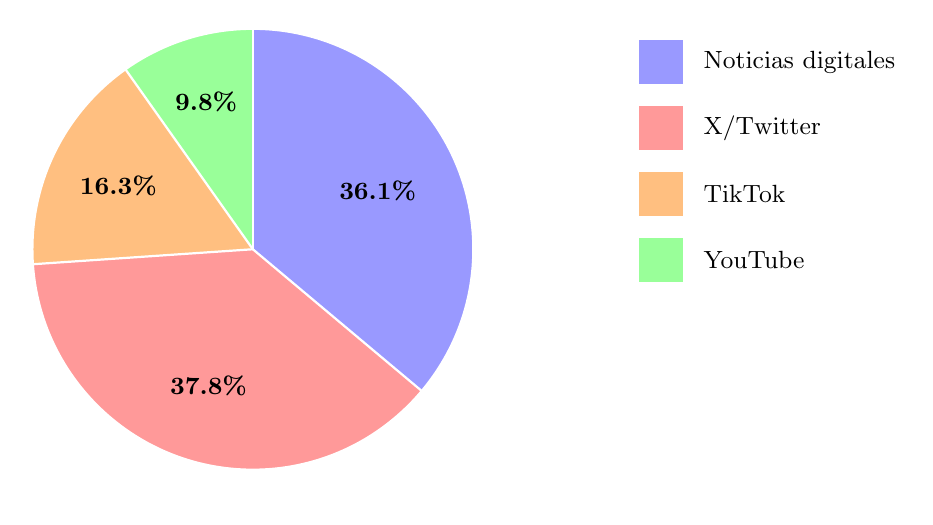
\begin{tikzpicture}[scale=1.4]
    \fill[blue!40]   (0,0) -- (90:2)     arc (90:-40:2)       -- cycle;
    \fill[red!40]    (0,0) -- (-40:2)    arc (-40:-176.1:2)   -- cycle;
    \fill[orange!50] (0,0) -- (-176.1:2) arc (-176.1:-234.7:2) -- cycle;
    \fill[green!40]  (0,0) -- (-234.7:2) arc (-234.7:-270:2)  -- cycle;

    \draw[thick, white] (0,0) circle (2);
    \foreach \a in {90,-40,-176.1,-234.7} {
        \draw[thick, white] (0,0) -- (\a:2);
    }

    % Etiquetas en el punto medio de cada sector
    \node[font=\small\bfseries] at (25:1.25)     {36.1\%};
    \node[font=\small\bfseries] at (-108:1.3)    {37.8\%};
    \node[font=\small\bfseries] at (-205.4:1.35) {16.3\%};
    \node[font=\small\bfseries] at (-252.4:1.4)  {9.8\%};

    % Leyenda
    \begin{scope}[shift={(3.5,1.5)}]
        \fill[blue!40]   (0,0)    rectangle (0.4,0.4);
        \fill[red!40]    (0,-0.6) rectangle (0.4,-0.2);
        \fill[orange!50] (0,-1.2) rectangle (0.4,-0.8);
        \fill[green!40]  (0,-1.8) rectangle (0.4,-1.4);
        \node[anchor=west, font=\small] at (0.5, 0.2)  {Noticias digitales};
        \node[anchor=west, font=\small] at (0.5,-0.4) {X/Twitter};
        \node[anchor=west, font=\small] at (0.5,-1.0) {TikTok};
        \node[anchor=west, font=\small] at (0.5,-1.6) {YouTube};
    \end{scope}
\end{tikzpicture}
}
        \caption[Distribución del corpus procesado por fuente de datos]{Distribución del corpus procesado por las cuatro fuentes de datos (noticias digitales, X/Twitter, YouTube y TikTok), mostrando el volumen relativo de cada canal.\\Fuente: Elaboración propia.}
        \label{5:fig7}
    \end{center}
\end{figure}

\begin{table}[h!]
    \caption[Cobertura del corpus procesado por canal de origen]{Distribución de los 40\,974 documentos del corpus procesado por canal de origen.}
    \label{5:table_fuente_gen}
    \centering
    \small
    \begin{tabular}{ m{5cm}M{2.5cm}M{2cm} }
        \specialrule{.1em}{.05em}{.05em}
        \Centering{Canal} & \Centering{Documentos} & \Centering{\%} \\
        \specialrule{.1em}{.05em}{.05em}
        X/Twitter      & 15\,495 & 37.8\% \\
        TikTok         & 6\,670  & 16.3\% \\
        RPP Noticias   & 5\,787  & 14.1\% \\
        Diario Correo  & 5\,568  & 13.6\% \\
        YouTube        & 4\,011  & 9.8\%  \\
        El Comercio    & 2\,424  & 5.9\%  \\
        La República   & 1\,019  & 2.5\%  \\
        \specialrule{.1em}{.05em}{.05em}
    \end{tabular}
    \begin{flushleft}
        \small Fuente: Elaboración propia, consulta al grafo de conocimiento.
    \end{flushleft}
\end{table}

\textbf{Universo filtrado por candidato.} Dado que el objeto de estudio es la
percepción mediática hacia los candidatos presidenciales, se aisló el subconjunto
de documentos que mencionan al menos a un candidato: 6\,293 documentos
(15.4\% del corpus total), que contienen 1\,282 temas distintos. Este subconjunto
constituye el universo analítico más relevante de la investigación, dado que
presenta un \textit{bleed} no político casi nulo: la categoría
\texttt{otros\_no\_politico} representa apenas el 0.4\% y deportes el 0\%,
resultando un corpus 94\% político-relevante. La proporción candidato/total crece
de forma sostenida hacia el cierre de campaña (de 6\% en enero a 25\% en abril),
confirmando la intensificación de la cobertura electoral. La distribución por
fuente de este subconjunto se reporta en la Tabla \ref{5:table_fuente_cand}.

\begin{table}[h!]
    \caption[Cobertura del corpus filtrado por candidato]{Distribución de los 6\,293 documentos que mencionan al menos un candidato presidencial, por canal de origen.}
    \label{5:table_fuente_cand}
    \centering
    \small
    \begin{tabular}{ m{5cm}M{2.5cm}M{2cm} }
        \specialrule{.1em}{.05em}{.05em}
        \Centering{Canal} & \Centering{Documentos} & \Centering{\%} \\
        \specialrule{.1em}{.05em}{.05em}
        X/Twitter      & 3\,086 & 49.0\% \\
        TikTok         & 1\,401 & 22.3\% \\
        YouTube        & 760    & 12.1\% \\
        RPP Noticias   & 459    & 7.3\%  \\
        Diario Correo  & 411    & 6.5\%  \\
        El Comercio    & 140    & 2.2\%  \\
        La República   & 36     & 0.6\%  \\
        \specialrule{.1em}{.05em}{.05em}
    \end{tabular}
    \begin{flushleft}
        \small Fuente: Elaboración propia, consulta al grafo de conocimiento.
    \end{flushleft}
\end{table}

En el universo filtrado por candidato, las redes sociales (X/Twitter, TikTok y
YouTube) concentran el 83\% de la cobertura, una dominancia mucho más marcada que
en el corpus general, lo que evidencia que la conversación electoral en torno a
los candidatos se desarrolla principalmente en plataformas sociales. La
distribución temática de este subconjunto, reportada en la Tabla
\ref{5:table_cat_cand}, está dominada por la categoría \texttt{institucional}
(42.9\%, principalmente debates y cobertura electoral), seguida por
\texttt{seguridad} (12.9\%) y \texttt{justicia\_legalidad} (11.4\%).

\begin{table}[h!]
    \caption[Distribución temática del corpus filtrado por candidato]{Distribución de los documentos que mencionan candidatos por categoría temática (top siete categorías).}
    \label{5:table_cat_cand}
    \centering
    \small
    \begin{tabular}{ m{5cm}M{2.5cm}M{2cm} }
        \specialrule{.1em}{.05em}{.05em}
        \Centering{Categoría} & \Centering{Documentos} & \Centering{\%} \\
        \specialrule{.1em}{.05em}{.05em}
        institucional        & 2\,701 & 42.9\% \\
        seguridad            & 809    & 12.9\% \\
        justicia\_legalidad  & 715    & 11.4\% \\
        corrupcion           & 535    & 8.5\%  \\
        social\_genero (encuestas) & 531 & 8.4\% \\
        economia             & 283    & 4.5\%  \\
        educacion            & 265    & 4.2\%  \\
        \specialrule{.1em}{.05em}{.05em}
    \end{tabular}
    \begin{flushleft}
        \small Fuente: Elaboración propia, consulta al grafo de conocimiento.
    \end{flushleft}
\end{table}

La variable dependiente del estudio —la percepción mediática hacia
cada candidato— se sintetiza en la Tabla \ref{5:table_cand_full} para los 40
candidatos presidenciales registrados. Por cada candidato se reportan cinco
indicadores obtenidos del grafo: el número de menciones en el corpus, la
cantidad de temas distintos que lo contienen, el número de medios (canales)
que lo cubren, el ratio menciones/tema y el sentimiento mediático promedio en
escala $[-1,1]$.

\begin{table}[h!]
    \caption[Indicadores mediáticos de los 40 candidatos presidenciales]{Menciones, temas distintos, medios de cobertura, ratio menciones/tema y sentimiento mediático promedio (escala $[-1,1]$) de los 40 candidatos presidenciales en el corpus procesado (1 ene -- 6 abr 2026).}
    \label{5:table_cand_full}
    \centering
    \scriptsize
    \begin{longtable}{ m{0.5cm}m{3.6cm}M{1.2cm}M{1.1cm}M{1.2cm}M{1.3cm}M{1.4cm} }
        \specialrule{.1em}{.05em}{.05em}
        \Centering{\#} & \Centering{Candidato} & \Centering{Menc.} & \Centering{Temas} & \Centering{Medios} & \Centering{Ratio M/T} & \Centering{Sent.} \\
        \specialrule{.1em}{.05em}{.05em}
        \endfirsthead
        \specialrule{.1em}{.05em}{.05em}
        \Centering{\#} & \Centering{Candidato} & \Centering{Menc.} & \Centering{Temas} & \Centering{Medios} & \Centering{Ratio M/T} & \Centering{Sent.} \\
        \specialrule{.1em}{.05em}{.05em}
        \endhead
        1  & Keiko Fujimori         & 1\,262 & 353 & 7 & 3.58 & $-0.193$ \\
        2  & Rafael López Aliaga    & 1\,025 & 321 & 7 & 3.19 & $-0.219$ \\
        3  & César Acuña            & 829 & 290 & 7 & 2.86 & $-0.335$ \\
        4  & Carlos Álvarez         & 515 & 168 & 7 & 3.07 & $+0.062$ \\
        5  & Alfonso López Chau     & 479 & 179 & 7 & 2.68 & $-0.162$ \\
        6  & Jorge Nieto Montesinos & 455 & 156 & 7 & 2.92 & $-0.046$ \\
        7  & Vladimir Cerrón        & 448 & 178 & 7 & 2.52 & $-0.406$ \\
        8  & Roberto Sánchez        & 369 & 159 & 7 & 2.32 & $-0.207$ \\
        9  & Fernando Olivera       & 349 & 97  & 7 & 3.60 & $-0.206$ \\
        10 & Marisol Pérez Tello    & 339 & 127 & 7 & 2.67 & $+0.106$ \\
        11 & José Luna Gálvez       & 317 & 151 & 7 & 2.10 & $-0.157$ \\
        12 & Enrique Valderrama     & 305 & 116 & 7 & 2.63 & $+0.015$ \\
        13 & Mario Vizcarra         & 267 & 102 & 7 & 2.62 & $-0.068$ \\
        14 & Wolfgang Grozo         & 245 & 98  & 7 & 2.50 & $-0.060$ \\
        15 & Mesías Guevara         & 242 & 102 & 7 & 2.37 & $+0.099$ \\
        16 & Yonhy Lescano          & 220 & 88  & 7 & 2.50 & $-0.083$ \\
        17 & José Williams Zapata   & 206 & 91  & 7 & 2.26 & $+0.092$ \\
        18 & George Forsyth         & 202 & 86  & 7 & 2.35 & $+0.111$ \\
        19 & Fiorella Molinelli     & 198 & 83  & 7 & 2.39 & $+0.059$ \\
        20 & Álvaro Paz de la Barra & 196 & 63  & 6 & 3.11 & $-0.054$ \\
        21 & Ronald Atencio         & 188 & 97  & 7 & 1.94 & $-0.077$ \\
        22 & Carlos Espá            & 168 & 76  & 7 & 2.21 & $+0.085$ \\
        23 & Rafael Belaúnde        & 142 & 81  & 6 & 1.75 & $+0.203$ \\
        24 & Roberto Chiabra        & 137 & 70  & 7 & 1.96 & $+0.154$ \\
        25 & Ricardo Belmont        & 133 & 59  & 6 & 2.25 & $+0.122$ \\
        26 & Alex Gonzáles          & 115 & 43  & 6 & 2.67 & $-0.001$ \\
        27 & Martín Vizcarra        & 115 & 65  & 7 & 1.77 & $-0.207$ \\
        28 & Herbert Caller         & 114 & 60  & 6 & 1.90 & $+0.113$ \\
        29 & Hernando de Soto       & 112 & 43  & 7 & 2.60 & $-0.034$ \\
        30 & Paul Jaimes            & 110 & 57  & 6 & 1.93 & $+0.047$ \\
        31 & Francisco Diez Canseco & 103 & 58  & 6 & 1.78 & $+0.035$ \\
        32 & Walter Chirinos        & 101 & 45  & 6 & 2.24 & $+0.045$ \\
        33 & Carlos Jaico           & 101 & 46  & 6 & 2.20 & $+0.239$ \\
        34 & Daniel Urresti         & 92  & 39  & 6 & 2.36 & $-0.135$ \\
        35 & Armando Massé          & 92  & 50  & 6 & 1.84 & $+0.227$ \\
        36 & Rosario Fernández Bazán & 88 & 51  & 6 & 1.73 & $+0.056$ \\
        37 & Charlie Carrasco       & 80  & 40  & 6 & 2.00 & $+0.086$ \\
        38 & Antonio Ortíz          & 78  & 39  & 6 & 2.00 & $+0.188$ \\
        39 & Antauro Humala         & 22  & 13  & 5 & 1.69 & $-0.433$ \\
        40 & Verónika Mendoza       & 10  & 9   & 5 & 1.11 & $-0.133$ \\
        \specialrule{.1em}{.05em}{.05em}
    \end{longtable}
    \begin{flushleft}
        \small Fuente: Elaboración propia, consulta al grafo de conocimiento.
    \end{flushleft}
\end{table}

De la Tabla \ref{5:table_cand_full} se desprenden tres lecturas relevantes para
caracterizar la cobertura mediática del proceso. En primer lugar, el
sentimiento es predominantemente negativo en los candidatos más
cubiertos —César Acuña ($-0.335$), Vladimir Cerrón ($-0.406$) y Antauro Humala
($-0.433$) son los más negativos—, mientras que solo un grupo de candidatos
de cobertura media presenta sentimiento neto positivo (Carlos Jaico $+0.239$,
Armando Massé $+0.227$, Rafael Belaúnde $+0.203$). En segundo lugar, el
número de medios funciona como indicador de alcance editorial: los 18
candidatos con mayor cobertura llegan a las 7 fuentes (cobertura universal),
mientras que los candidatos marginales descienden a 6 o 5 medios (Antauro
Humala y Verónika Mendoza), evidenciando un menor alcance mediático. En tercer
lugar, el ratio menciones/tema distingue entre candidatos con narrativa
mediática construida y candidatos de aparición incidental: valores altos
($>3.0$, como Fernando Olivera 3.60, Keiko Fujimori 3.58 o Rafael López Aliaga
3.19) indican cobertura insistente y repetida sobre la agenda propia del
candidato, mientras que valores bajos ($<1.9$, como Verónika Mendoza 1.11 o
Antauro Humala 1.69) reflejan menciones dispersas y esporádicas donde cada
aparición corresponde a un tema casi distinto, propio de candidatos mencionados
de pasada y no como protagonistas.

\subsection*{Contraste y Validación de la Hipótesis Específica 2 (HE2)}
La Hipótesis Específica 2 planteaba que el uso de un módulo híbrido basado en Modelos de Lenguaje de Gran Escala (LLM) y arquitecturas de recuperación avanzadas permitiría alcanzar un desempeño óptimo caracterizado por una métrica $F1 \ge 0.80$ y un error absoluto medio ($MAE \le 0.15$) en tareas de clasificación y extracción.

Al contrastar los datos empíricos recopilados durante la fase de evaluación, se obtuvieron los siguientes indicadores consolidados:
\begin{itemize}
    \item Error Absoluto Medio logrado: $\text{MAE} = 0.107$, el cual cumple con la condición matemática establecida ($\text{MAE}_{\text{logrado}} \le 0.15$).
    \item Métrica de precisión armónica: $F1\text{-score} \ge 0.825$ sostenido en todas las tareas críticas de extracción (categorización, identificación de candidatos, deduplicación de temas y extracción de actores), superando sistemáticamente el umbral base fijado ($F1_{\text{logrado}} \ge 0.80$).
\end{itemize}

\noindent \textbf{Dictamen de Validación:} Al haberse verificado simultáneamente ambas condiciones paramétricas dentro de los entornos de prueba correspondientes a la arquitectura Medallion y el pipeline optimizado con DeepSeek-Chat, \textbf{se acepta formalmente la Hipótesis Específica 2 (HE2)}.

% ──────────────────────────────────────────────────────────────
\section{Despliegue}
% ──────────────────────────────────────────────────────────────

\textbf{Actividad 1: Desplegar el servidor MCP de inteligencia electoral}
\\
Se diseñó e implementó la interfaz del sistema de inteligencia electoral como un
\textbf{servidor MCP} (\textit{Model Context Protocol}) sobre transporte
\texttt{streamable-http}, desplegado en contenedor Docker en la misma red local
que las bases de datos PostgreSQL y Neo4j (\textit{stack} reproducible en una
\textit{laptop} o servidor único, sin servicios cloud gestionados). El servidor
\texttt{electoral\_mcp} se implementa en Python 3.12 con \texttt{FastMCP 3.2.4}
sobre \texttt{Starlette} y \texttt{uvicorn}, autenticación \textit{Bearer token}
y \textit{lifespan} combinado que conecta los \textit{pools} \texttt{asyncpg} y
\texttt{neo4j async} antes del primer \textit{request}. La interacción con el
sistema se realiza desde clientes MCP estándar (Claude Desktop, Claude.ai web o
Cursor) que descubren las 14 herramientas tipadas y las invocan en lenguaje
natural; para presentaciones remotas se expone vía \texttt{cloudflared tunnel} o
\texttt{ngrok} sobre HTTPS efímero. La arquitectura del prototipo integrado se
muestra en la Figura \ref{5:fig24}.

\begin{figure}[!ht]
    \begin{center}
        \resizebox{0.85\textwidth}{!}{\input{4/figures/fig24_demo_flux}}
        \caption[Proceso de operación del prototipo del sistema de inteligencia electoral]{Proceso de operación del prototipo: ingesta diaria del corpus multifuente, etiquetado LLM, sincronización del grafo y consultas en lenguaje natural desde un cliente MCP que invoca las 14 herramientas tipadas del servidor \texttt{electoral\_mcp}.\\
            Fuente: Elaboración propia.}
        \label{5:fig24}
    \end{center}
\end{figure}

\textbf{Actividad 2: Ejecutar prototipo con datos electorales en vivo}
\\
Durante esta actividad se materializaron los flujos de la arquitectura del
prototipo presentados en la figura previa. La prueba piloto se llevó a cabo
poniendo el sistema en operación durante una semana de campaña electoral en pleno
desarrollo —que incluyó un debate presidencial—. El orquestador diario
(\texttt{run-day}/\texttt{run-range}) procesó día tras día las cuatro fuentes de
datos con concurrencia intra-batch (\texttt{BATCH\_SIZE=5}), produciendo los
indicadores ISN, IRT e IVE de los candidatos en contienda y refrescando las
vistas Gold materializadas (\texttt{gold\_sentimiento\_diario},
\texttt{gold\_temas\_diarios}, \texttt{gold\_cobertura\_medios}) que sirven de
fuente al servidor MCP. Los principales hallazgos de la prueba piloto se exponen
en la Figura \ref{5:fig25}.

\begin{figure}[!ht]
    \begin{center}
        \includegraphics[width=0.85\textwidth]{4/figures/fig25_piloto.png}
        \caption[Resultados del prototipo durante la prueba piloto del 12 y 13 de marzo de 2026]{Resultados del prototipo de inteligencia electoral durante la prueba piloto de los días 12 y 13 de marzo de 2026, mostrando la evolución del ISN por candidato y los temas emergentes identificados en la cobertura mediática, todos consultados desde un cliente MCP mediante las herramientas \texttt{evolucion\_sentimiento\_candidato}, \texttt{temas\_top\_periodo} y \texttt{panorama\_diario}.\\Fuente: Elaboración propia.}
        \label{5:fig25}
    \end{center}
\end{figure}

La prueba piloto confirmó la viabilidad del sistema para detectar cambios
relevantes en la percepción proyectada por los medios —como el pico de sentimiento negativo
registrado durante y después del debate presidencial— y para identificar los
temas que emergieron como consecuencia de los intercambios entre candidatos. El
sistema también identificó correctamente una discrepancia significativa entre la
cobertura positiva de un candidato en los medios digitales y el sentimiento
negativo expresado hacia ese mismo candidato en X/Twitter durante la misma
semana, constituyendo un hallazgo de inteligencia electoral relevante para los
analistas usuarios del sistema.

Como caso de uso real del sistema, se realizó la siguiente consulta al servidor
MCP desde un cliente LLM en lenguaje natural:

\begin{quote}
\textit{``Muéstrame qué candidato presidencial Perú 2026 tuvo la mayor caída de
sentimiento mediático entre el 10 y 12 de marzo. Dame: 1) cuánto bajó, 2) la razón
principal según las noticias, 3) las 2 noticias más negativas con titular, medio
y URL. Visualiza la evolución día a día.''}
\end{quote}

A partir de esta consulta, el LLM cliente seleccionó automáticamente las
herramientas \texttt{comparar\_candidatos\_sentimiento},
\texttt{noticias\_por\_actor} y \texttt{citar\_evidencia} con sus parámetros
tipados, ejecutó las consultas SQL/Cypher subyacentes contra Postgres y Neo4j, y
construyó la respuesta fundamentada en evidencia textual del corpus. El resultado
se muestra en la Figura \ref{5:fig26}.

\begin{figure}[!ht]
    \centering
    \begin{subfigure}{0.85\textwidth}
        \centering
        \includegraphics[width=\linewidth]{4/figures/fig12a_evolucion_sentimiento.png}
        \caption{Evolución del sentimiento mediático día a día del candidato con la mayor caída entre el 10 y 12 de marzo de 2026.}
        \label{5:fig26a}
    \end{subfigure}
    \\[0.5cm]
    \begin{subfigure}{0.85\textwidth}
        \centering
        \includegraphics[width=\linewidth]{4/figures/fig12b_noticias_razones.png}
        \caption{Las dos noticias más negativas que el sistema cita como razones de la caída, con titular, medio y URL.}
        \label{5:fig26b}
    \end{subfigure}
    \caption[Consulta GraphRAG en lenguaje natural sobre la mayor caída de sentimiento mediático entre el 10 y 12 de marzo de 2026]{Respuesta del sistema GraphRAG a la consulta en lenguaje natural sobre la mayor caída de sentimiento mediático de un candidato presidencial entre el 10 y 12 de marzo de 2026: (a) evolución del ISN día a día con la magnitud y dirección de la caída, y (b) las dos noticias más negativas del corpus original que el sistema cita como razones de la caída, con su medio de origen y URL.\\Fuente: Elaboración propia.}
    \label{5:fig26}
\end{figure}